\documentclass[letterpaper]{article}

\usepackage{cite}
\usepackage[utf8]{inputenc}
\usepackage{graphicx}
\usepackage{hyperref}
\usepackage{amsmath,amsthm,amssymb,mathtools}
\usepackage{prftree}

\usepackage{tikz}
\usetikzlibrary{calc,positioning,fit,shapes}

\newcommand{\todo}[1]{{\color{red}[TODO: #1]}}

\begin{document}

\section{Language Design}

The language has the following design goals:

\begin{itemize}
\item A useful foundational set of parser primitives and combinators,
\item A capacity to capture context-sensitivity and data-dependency
  via a constraint system, and
\item  A module system that enables nested grammars and composes with
  the constraint system.
\end{itemize}

\begin{itemize}
\item The core structure of a Parsley specification is provided by a
  {\em parsing expression grammar (PEG)} \cite{ford2004popl},
  specified in notation similar to  {\em extended BNF (EBNF)} for
  grammar productions.  Although {\em context-free grammars (CFGs)}
  use the EBNF notation, there are critical differences in the PEG
  notation: (a) the choice combinator in PEGs is ordered, as opposed
  to non-deterministic in CFGs, and (b) the PEG notation includes
  syntactic predicates that do not occur in CFGs.  The choice of a PEG
  core provides us the set of primitives and combinators as we desire.

\item Context management is provided by a fairly traditional
  attribute-grammar system, where the expression language for
  attribute computations is purely functional and strongly-typed.  In
  Parsley, non-terminals have user-defined attributes, while terminals
  have a default attribute value of type byte or byte-string.  This
  provides us with the tools needed to capture context-sensitivity.

\item Additional context-sensitivity is provided by a constraint
  system that guards further processing  within a non-terminal production.
  The constraint language uses the attribute system to perform
  context-sensitive checks, and employs primitives in the constraint
  expression language to perform data-dependent parsing.

\item A module system allows the composition of independent grammars.
\end{itemize}

The expression sublanguage used in attribute updates and constraints
is a strongly typed polymorphic functional language supporting
user-defined types and functions.  It includes a standard library of
common types and utility functions.  The expression and data type
sublanguage is  designed to ensure that recursive and
iterative computations always terminate.

\section{Abstract syntax}

\begin{figure}
  \begin{tabular}{l c l l}
    Paths        & $p$      & ::= & $x\ |\ x.p$ \\
    Constants    & c        & ::= & 0,1,\ldots\ $|$\ 'A', 'B', \ldots\ $|$\ \ldots \\
    Attributes   & $l$      & ::= & $l^i\ |\ l^s$ \\
    Base types   & $\nu$    & ::= & $ \texttt{unit}\ |\ \texttt{uint8}\ |\ \texttt{int32}\ |\ \ldots\ $ \\
    Types        & $\tau$   & ::= & $\alpha\ |\ \nu\ |\ (\tau_i)\ |\ \tau\rightarrow\tau\ |\ \texttt{typeof}(N)$ \\
                 &          &     & $|\ \sum_i C_i\tau_i\ |\ \prod_i \{l_i:\tau_i\}\ $ \\
    Schemes      & $\sigma$ & ::= & $\forall\alpha.\tau$ \\
    Expressions  & $e$      & ::= & $p\ |\ \textrm{c}\ |\ (e_i)\ |\ e\ e\ |\ e\ \texttt{op}\ e\ |\ e.l\ |\ \ldots\ $ \\
    Statements   & $s$      & ::= & $ p = e $ \\
                 &          &     & \\
    Constraints  & $\phi$   & ::= & $ e $ \\
    Actions      & $a$      & ::= & $ {s_i} $ \\
    Rules        & $r$      & ::= & $ \epsilon\ |\ \textrm{c}\ |\ \phi\ |\ (x=)^?N\{l_i=e_i\}$ \\
                 &          &     & $|\ r\ r\ |\ r\ /\ r\ |\ r^{*e?}\ |\ !r\ |\ !^Rr\ |\ a$ \\
    Productions  & $P$      & ::= & $ N\{l_i:\tau_i\} := r$ \\
    Format       & $F$      & ::= & $ \{ \tau_i, N\{l_i:\tau_i\}, P_i \}$ \\
  \end{tabular}
  \caption{Abstract Syntax of the Parsley specification language}
  \label{f:parsley-syntax}
\end{figure}

\todo{add missing expressions.}

The abstract syntax elements of Parsley are displayed in
Figure~\ref{f:parsley-syntax}, where $\alpha$ ranges over type
variables, $x$ over identifiers, $op$ over standard arithmetic and
boolean operators, and $l$ over inherited $l^i$ and synthesized $l^s$
attributes.  Paths are used to  access attributes from named syntax
elements: $x.l$ accesses the $l$ attribute of the $x$-named occurrence
of non-terminal $(x=N)$ in a rule $r$, enabling attributes to be used
in constraint expressions and action statements.  Paths are also used
to support the module system (not shown) enabling cross-module use of
types and syntax elements.

The type system is a conventional polymorphic functional type system
with records. Constraints are expressions with Boolean type.  The
Parsley library has standard data types such as polymorphic lists,
sets, and maps.  The expression language is also conventional, with
some elements such as pattern matching and let binding constructs (not
shown).  A record type $\texttt{typeof}(N)$ is used to represent a
non-terminal $N$, with the record fields corresponding to the
attributes of the non-terminal.

The core grammatical constructs are the actions, rules, productions,
and formats.  These are based on parsing expression grammars (PEGs)
\cite{ford2004popl}, extended with an attribute system and
constraints to capture context sensitivity.  Rules correspond closely to
the expressions of PEGs, but with some extensions.  $r\ r$ denotes the
PEG sequence operator, while $r\ /\ r$ is the PEG ordered choice.  The
$!r$ construct is the \emph{not} syntactic predicate in PEG.  The
$N\{l_i=e_i\}$ rule expands the $N$ non-terminal after initializing
its inherited attributes. $r^{*e?}$ denotes the Kleene star, but with
an optional bound $e$ that is context sensitive.  A constraint $\phi$
is a Parsley extension of PEG, and could be thought of as a
\emph{contextual} predicate: it checks the context, typically using
the attribute values of syntactic elements in the current context, and
decides whether the current parsing alternative can continue.  The
action rule $a$ typically sets the values of synthesized attributes
of the non-terminal of the current production and continues the parse.

Parsley is equipped with a module system that enables splitting a
specification into multiple files, allowing data specifications to be
re-used in different contexts.

\subsection*{Extensions under development}

\begin{figure*}[!ht]
  \centering
  \resizebox{10cm}{!}{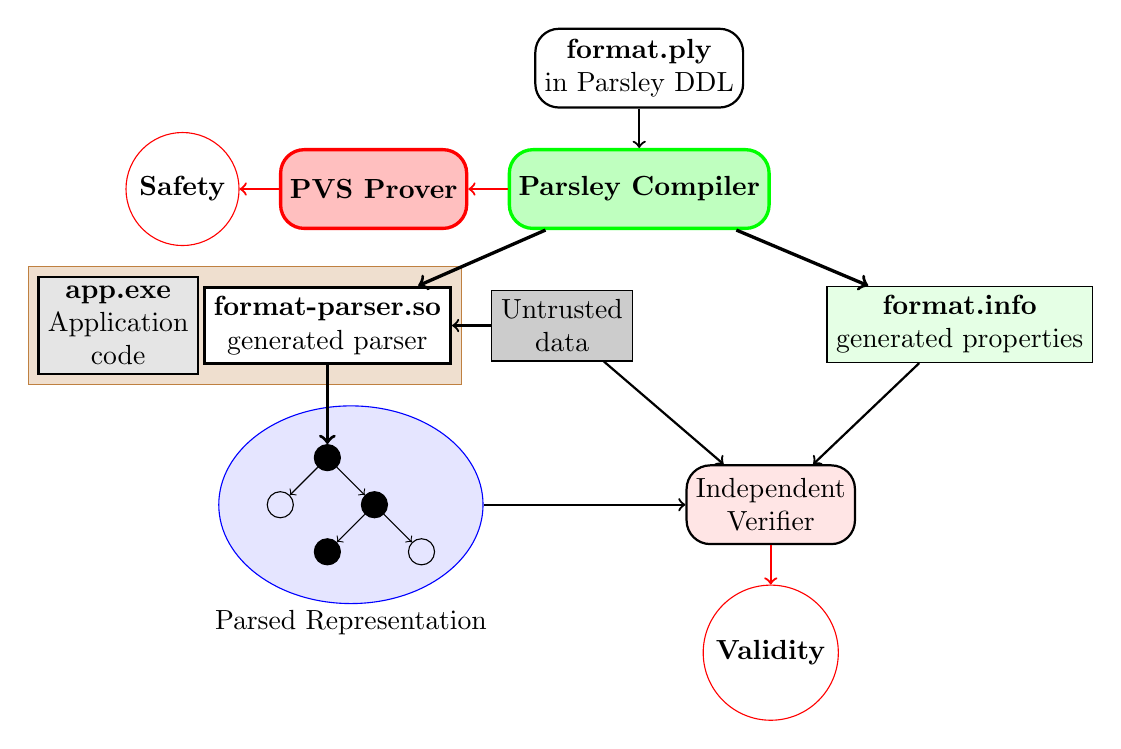
\begin{tikzpicture}[
    node distance=5mm,
    align=center,
    spec/.style={rectangle, rounded corners=3mm, minimum size=10mm, draw=black, thick},
    info/.style={rectangle, draw=black, fill=green!10!white},
    lib/.style={rectangle, very thick, draw=black, fill=white},
    app/.style={rectangle, thick, draw=black, fill=black!10!white},
    prog/.style={rectangle, draw=brown, fill=brown!25!white},
    compiler/.style={rectangle, rounded corners=3mm, minimum size=10mm,
      very thick, draw=green, fill=green!25!white},
    prover/.style={rectangle, rounded corners=3mm, minimum size=10mm,
      very thick, draw=red, fill=red!25!white},
    verifier/.style={rectangle, rounded corners=3mm, minimum size=10mm,
      thick, draw=black, fill=red!10!white},
    data/.style={rectangle, draw=black, fill=black!20!white},
    prop/.style={circle, draw=red},
    ast/.style={circle, draw=black},
    memory/.style={ellipse, draw=blue, fill=blue!10!white},
    input/.style={->, thick, black},
    gen/.style={->, very thick, black},
    proverinput/.style={->, thick, red},
    proveroutput/.style={->, thick, red},
    tree/.style={->, black},
  ]

  \pgfdeclarelayer{background}
  \pgfdeclarelayer{main}
  \pgfdeclarelayer{foreground}
  \pgfsetlayers{background,main,foreground}

  % main pipeline
  \begin{pgfonlayer}{main}
    \node (spec)      [spec]                         {\textbf{format.ply}\\ in Parsley DDL};

    \node (compiler)  [compiler, below=of spec]      {\textbf{Parsley Compiler}};

    \node (prover)    [prover, left=of compiler]     {\textbf{PVS Prover}};

    \node (safety)    [prop,left=of prover]          {\textbf{Safety}};

    \node (lib)       [lib, below left=1cm of compiler]   {\textbf{format-parser.so}\\ generated parser};

    \node (info)      [info, below right=1cm of compiler] {\textbf{format.info}\\ generated properties};

    \node (app)       [app, left=0.5mm of lib]       {\textbf{app.exe}\\ Application\\ code};

    \node (data)      [data, right=of lib]           {Untrusted\\ data};
  \end{pgfonlayer}

  % complete application
  \begin{pgfonlayer}{background}
    \node (prog)      [prog, fit=(app.south west) (app.north west)
                                 (lib.south east) (lib.north east)] {};
  \end{pgfonlayer}

  % generated AST in memory
  \begin{pgfonlayer}{main}
    \node (root)      [ast, fill=black, below] at ($(lib.south)+(0,-1cm)$)  {};

    \node (c0)        [ast, below left=of root] {};
    \node (c1)        [ast, below right=of root, fill=black] {};
    \node (c10)       [ast, below left=of c1, fill=black] {};
    \node (c11)       [ast, below right=of c1] {};
  \end{pgfonlayer}
  \begin{pgfonlayer}{background}
    \node (tree)      [memory, fit=(root) (c0) (c1) (c10) (c11)] {};
  \end{pgfonlayer}

  \begin{pgfonlayer}{main}
    \node (appdata)   [below=-0.5mm of tree] {Parsed Representation};
    \node (verifier)  [verifier] at (compiler.south east |- tree) {Independent\\Verifier};
    \node (validity)  [prop, below=of verifier] {\textbf{Validity}};
  \end{pgfonlayer}

  % flow
  \draw[input]         (spec) -- (compiler);
  \draw[gen]           (compiler) -- (lib);
  \draw[gen]           (compiler) -- (info);
  \draw[proverinput]   (compiler) -- (prover);
  \draw[proveroutput]  (prover) -- (safety);

  \draw[input]         (data) -- (lib);

  \draw[gen]           (lib) -- (root);
  \draw[tree]          (root) -- (c0);
  \draw[tree]          (root) -- (c1);
  \draw[tree]          (c1) -- (c10);
  \draw[tree]          (c1) -- (c11);

  \draw[input]         (tree) -- (verifier);
  \draw[input]         (info) -- (verifier);
  \draw[input]         (data) -- (verifier);
  \draw[proveroutput]  (verifier) -- (validity);

\end{tikzpicture}
}
  \label{f:pipeline}
  \caption{Parsley in context.}
\end{figure*}

The Parsley language is a work-in-progress, and is being adapted as we
attempt to use it to capture more data formats.  The parsing of a PDF
file involves seeking to the end of the file (or a specific marker)
and searching backwards for a syntactic element.  This motivated the
$!^Rr$ construct, which can be considered as a \emph{reverse-not}
predicate: it checks backwards from the current parsing location
whether the parse buffer matches $r$.

We are also considering extending Parsley with primitives to capture
manipulations of the current parsing offset by actions such as
seeking.  Such offset manipulation could either derive declaratively
from the format specification, or procedurally under the control of
the application driving the parser.  A design challenge is to ensure
both types of manipulations are supported and compose well.  In
addition, this is one of the most security-critical aspects of
parsing: ensuring that offsets derived from untrusted data are used in
valid ways.

\section{Type system}

Figure~\ref{f:ctxt} defines a typing context, and shows the mutually
recursive well-formed judgments for a context $\vdash\Gamma$ and a
type $\Gamma\vdash\tau$.

\begin{figure}
    \begin{tabular}{l c l l}
    Typing contexts        & $\Gamma$      & ::= & $\cdot\ |\ \Gamma, \alpha\ |\ \Gamma, x: \tau\ |\ \Gamma, N: \{l_i:\tau_i\}$ \\
  \end{tabular}

  $$ \boxed{\vdash\Gamma} \qquad \boxed{\Gamma\vdash\tau} $$
  $$ \prftree{\prfassumption{\alpha\notin\Gamma}}
             {\vdash\Gamma, \alpha}\qquad
     \prftree{\prfassumption{x\notin\Gamma}}{\prfassumption{\Gamma\vdash\tau}}
             {\vdash\Gamma, x:\tau}\qquad
     \prftree{\prfassumption{N\notin\Gamma}}{\prfassumption{\Gamma\vdash\{l_i:\tau_i\}}}
             {\vdash\Gamma, N:\{l_i:\tau_i\}} $$
  $$ \prfaxiom{\Gamma\vdash\nu}\qquad
     \prftree{\prfassumption{\alpha\in\Gamma}}
             {\Gamma\vdash\alpha}\qquad
     \prftree{\prfassumption{\Gamma\vdash\tau_i}}
             {\Gamma\vdash(\tau_i)}\qquad
     \prftree{\prfassumption{\Gamma\vdash\tau_a}}{\prfassumption{\Gamma\vdash\tau_b}}
             {\Gamma\vdash\tau_a\rightarrow\tau_b}\qquad
     \prftree{\prfassumption{N\in\Gamma}}
             {\texttt{typeof}(N)} $$
  $$ \prftree{\prfassumption{C_i=C_j\Rightarrow i=j}}{\prfassumption{\Gamma\vdash\tau_i}}
             {\Gamma\vdash\sum_i C_i\tau_i}\qquad
     \prftree{\prfassumption{\Gamma\vdash\tau_i}}{\prfassumption{l_i=l_j\Rightarrow i=j}}
             {\Gamma\vdash\{l_i:\tau_i\}}\qquad
     \prftree{\prfassumption{\beta\notin\Gamma; \Gamma,\beta\vdash[\alpha\rightarrow\beta]\tau}}
             {\Gamma\vdash\forall\alpha.\tau} $$
  \caption{Typing judgements}
  \label{f:ctxt}
\end{figure}

\todo{adding paths and path resolution.}

\section*{Acknowledgments}
This work was supported by DARPA under agreement number HR001119C0075.
The views and conclusions contained herein are those of the authors
and should not be interpreted as necessarily representing the official
policies or endorsements, either expressed or implied, of DARPA or the
U.S. Government.

\bibliographystyle{plain}
\bibliography{parsley}
\end{document}
